% Created by tikzDevice version 0.12.6 on 2024-04-11 10:03:48
% !TEX encoding = UTF-8 Unicode
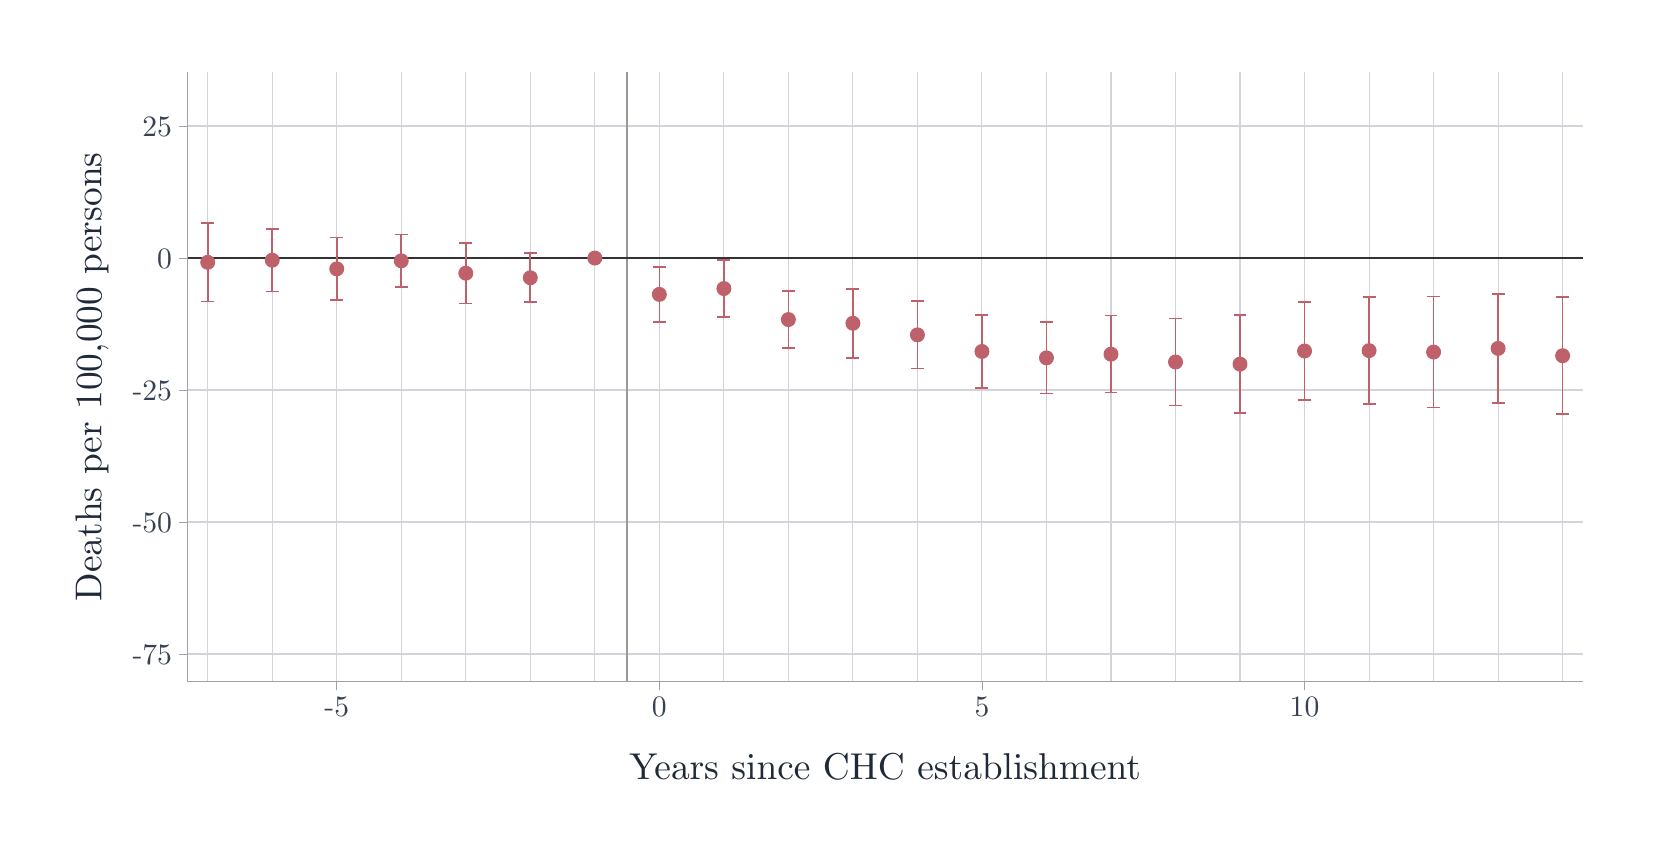
\begin{tikzpicture}[x=1pt,y=1pt]
\definecolor{fillColor}{RGB}{255,255,255}
\path[use as bounding box,fill=fillColor] (0,0) rectangle (578.16,289.08);
\begin{scope}
\path[clip] (  0.00,  0.00) rectangle (578.16,289.08);
\definecolor{drawColor}{RGB}{255,255,255}

\path[draw=drawColor,line width= 0.6pt,line join=round,line cap=round,fill=fillColor] ( -0.00,  0.00) rectangle (578.16,289.08);
\end{scope}
\begin{scope}
\path[clip] ( 57.55, 52.74) rectangle (562.16,273.08);
\definecolor{drawColor}{RGB}{255,255,255}
\definecolor{fillColor}{RGB}{255,255,255}

\path[draw=drawColor,line width= 0.6pt,line join=round,line cap=round,fill=fillColor] ( 57.55, 52.74) rectangle (562.16,273.08);
\definecolor{drawColor}{RGB}{209,213,219}

\path[draw=drawColor,line width= 0.4pt,line join=round] ( 65.05, 52.74) --
	( 65.05,273.08);

\path[draw=drawColor,line width= 0.4pt,line join=round] ( 88.37, 52.74) --
	( 88.37,273.08);

\path[draw=drawColor,line width= 0.4pt,line join=round] (135.00, 52.74) --
	(135.00,273.08);

\path[draw=drawColor,line width= 0.4pt,line join=round] (158.31, 52.74) --
	(158.31,273.08);

\path[draw=drawColor,line width= 0.4pt,line join=round] (181.62, 52.74) --
	(181.62,273.08);

\path[draw=drawColor,line width= 0.4pt,line join=round] (204.94, 52.74) --
	(204.94,273.08);

\path[draw=drawColor,line width= 0.4pt,line join=round] (251.57, 52.74) --
	(251.57,273.08);

\path[draw=drawColor,line width= 0.4pt,line join=round] (274.88, 52.74) --
	(274.88,273.08);

\path[draw=drawColor,line width= 0.4pt,line join=round] (298.20, 52.74) --
	(298.20,273.08);

\path[draw=drawColor,line width= 0.4pt,line join=round] (321.51, 52.74) --
	(321.51,273.08);

\path[draw=drawColor,line width= 0.4pt,line join=round] (368.14, 52.74) --
	(368.14,273.08);

\path[draw=drawColor,line width= 0.4pt,line join=round] (391.45, 52.74) --
	(391.45,273.08);

\path[draw=drawColor,line width= 0.4pt,line join=round] (414.77, 52.74) --
	(414.77,273.08);

\path[draw=drawColor,line width= 0.4pt,line join=round] (438.08, 52.74) --
	(438.08,273.08);

\path[draw=drawColor,line width= 0.4pt,line join=round] (484.71, 52.74) --
	(484.71,273.08);

\path[draw=drawColor,line width= 0.4pt,line join=round] (508.02, 52.74) --
	(508.02,273.08);

\path[draw=drawColor,line width= 0.4pt,line join=round] (531.34, 52.74) --
	(531.34,273.08);

\path[draw=drawColor,line width= 0.4pt,line join=round] (554.65, 52.74) --
	(554.65,273.08);

\path[draw=drawColor,line width= 0.4pt,line join=round] ( 57.55, 62.76) --
	(562.16, 62.76);

\path[draw=drawColor,line width= 0.4pt,line join=round] ( 57.55,110.45) --
	(562.16,110.45);

\path[draw=drawColor,line width= 0.4pt,line join=round] ( 57.55,158.14) --
	(562.16,158.14);

\path[draw=drawColor,line width= 0.4pt,line join=round] ( 57.55,205.83) --
	(562.16,205.83);

\path[draw=drawColor,line width= 0.4pt,line join=round] ( 57.55,253.53) --
	(562.16,253.53);

\path[draw=drawColor,line width= 0.4pt,line join=round] (111.68, 52.74) --
	(111.68,273.08);

\path[draw=drawColor,line width= 0.4pt,line join=round] (228.25, 52.74) --
	(228.25,273.08);

\path[draw=drawColor,line width= 0.4pt,line join=round] (344.82, 52.74) --
	(344.82,273.08);

\path[draw=drawColor,line width= 0.4pt,line join=round] (461.40, 52.74) --
	(461.40,273.08);
\definecolor{drawColor}{gray}{0.60}

\path[draw=drawColor,line width= 0.6pt,line join=round] (216.60, 52.74) -- (216.60,273.08);
\definecolor{drawColor}{gray}{0.20}

\path[draw=drawColor,line width= 0.6pt,line join=round] ( 57.55,205.83) -- (562.16,205.83);
\definecolor{drawColor}{RGB}{191,97,106}
\definecolor{fillColor}{RGB}{191,97,106}

\path[draw=drawColor,line width= 0.4pt,line join=round,line cap=round,fill=fillColor] ( 65.05,204.29) circle (  2.50);

\path[draw=drawColor,line width= 0.4pt,line join=round,line cap=round,fill=fillColor] ( 88.37,205.05) circle (  2.50);

\path[draw=drawColor,line width= 0.4pt,line join=round,line cap=round,fill=fillColor] (111.68,201.93) circle (  2.50);

\path[draw=drawColor,line width= 0.4pt,line join=round,line cap=round,fill=fillColor] (135.00,204.83) circle (  2.50);

\path[draw=drawColor,line width= 0.4pt,line join=round,line cap=round,fill=fillColor] (158.31,200.35) circle (  2.50);

\path[draw=drawColor,line width= 0.4pt,line join=round,line cap=round,fill=fillColor] (181.62,198.71) circle (  2.50);

\path[draw=drawColor,line width= 0.4pt,line join=round,line cap=round,fill=fillColor] (228.25,192.70) circle (  2.50);

\path[draw=drawColor,line width= 0.4pt,line join=round,line cap=round,fill=fillColor] (251.57,194.81) circle (  2.50);

\path[draw=drawColor,line width= 0.4pt,line join=round,line cap=round,fill=fillColor] (274.88,183.60) circle (  2.50);

\path[draw=drawColor,line width= 0.4pt,line join=round,line cap=round,fill=fillColor] (298.20,182.26) circle (  2.50);

\path[draw=drawColor,line width= 0.4pt,line join=round,line cap=round,fill=fillColor] (321.51,178.08) circle (  2.50);

\path[draw=drawColor,line width= 0.4pt,line join=round,line cap=round,fill=fillColor] (344.82,172.07) circle (  2.50);

\path[draw=drawColor,line width= 0.4pt,line join=round,line cap=round,fill=fillColor] (368.14,169.76) circle (  2.50);

\path[draw=drawColor,line width= 0.4pt,line join=round,line cap=round,fill=fillColor] (391.45,171.10) circle (  2.50);

\path[draw=drawColor,line width= 0.4pt,line join=round,line cap=round,fill=fillColor] (414.77,168.27) circle (  2.50);

\path[draw=drawColor,line width= 0.4pt,line join=round,line cap=round,fill=fillColor] (438.08,167.50) circle (  2.50);

\path[draw=drawColor,line width= 0.4pt,line join=round,line cap=round,fill=fillColor] (461.40,172.24) circle (  2.50);

\path[draw=drawColor,line width= 0.4pt,line join=round,line cap=round,fill=fillColor] (484.71,172.38) circle (  2.50);

\path[draw=drawColor,line width= 0.4pt,line join=round,line cap=round,fill=fillColor] (508.02,171.86) circle (  2.50);

\path[draw=drawColor,line width= 0.4pt,line join=round,line cap=round,fill=fillColor] (531.34,173.18) circle (  2.50);

\path[draw=drawColor,line width= 0.4pt,line join=round,line cap=round,fill=fillColor] (554.65,170.54) circle (  2.50);

\path[draw=drawColor,line width= 0.4pt,line join=round,line cap=round,fill=fillColor] (204.94,205.83) circle (  2.50);

\path[draw=drawColor,line width= 0.6pt,line join=round] ( 62.72,218.44) --
	( 67.38,218.44);

\path[draw=drawColor,line width= 0.6pt,line join=round] ( 65.05,218.44) --
	( 65.05,190.14);

\path[draw=drawColor,line width= 0.6pt,line join=round] ( 62.72,190.14) --
	( 67.38,190.14);

\path[draw=drawColor,line width= 0.6pt,line join=round] ( 86.04,216.39) --
	( 90.70,216.39);

\path[draw=drawColor,line width= 0.6pt,line join=round] ( 88.37,216.39) --
	( 88.37,193.71);

\path[draw=drawColor,line width= 0.6pt,line join=round] ( 86.04,193.71) --
	( 90.70,193.71);

\path[draw=drawColor,line width= 0.6pt,line join=round] (109.35,213.30) --
	(114.01,213.30);

\path[draw=drawColor,line width= 0.6pt,line join=round] (111.68,213.30) --
	(111.68,190.56);

\path[draw=drawColor,line width= 0.6pt,line join=round] (109.35,190.56) --
	(114.01,190.56);

\path[draw=drawColor,line width= 0.6pt,line join=round] (132.66,214.40) --
	(137.33,214.40);

\path[draw=drawColor,line width= 0.6pt,line join=round] (135.00,214.40) --
	(135.00,195.26);

\path[draw=drawColor,line width= 0.6pt,line join=round] (132.66,195.26) --
	(137.33,195.26);

\path[draw=drawColor,line width= 0.6pt,line join=round] (155.98,211.33) --
	(160.64,211.33);

\path[draw=drawColor,line width= 0.6pt,line join=round] (158.31,211.33) --
	(158.31,189.38);

\path[draw=drawColor,line width= 0.6pt,line join=round] (155.98,189.38) --
	(160.64,189.38);

\path[draw=drawColor,line width= 0.6pt,line join=round] (179.29,207.55) --
	(183.96,207.55);

\path[draw=drawColor,line width= 0.6pt,line join=round] (181.62,207.55) --
	(181.62,189.86);

\path[draw=drawColor,line width= 0.6pt,line join=round] (179.29,189.86) --
	(183.96,189.86);

\path[draw=drawColor,line width= 0.6pt,line join=round] (225.92,202.65) --
	(230.58,202.65);

\path[draw=drawColor,line width= 0.6pt,line join=round] (228.25,202.65) --
	(228.25,182.74);

\path[draw=drawColor,line width= 0.6pt,line join=round] (225.92,182.74) --
	(230.58,182.74);

\path[draw=drawColor,line width= 0.6pt,line join=round] (249.24,205.10) --
	(253.90,205.10);

\path[draw=drawColor,line width= 0.6pt,line join=round] (251.57,205.10) --
	(251.57,184.52);

\path[draw=drawColor,line width= 0.6pt,line join=round] (249.24,184.52) --
	(253.90,184.52);

\path[draw=drawColor,line width= 0.6pt,line join=round] (272.55,193.90) --
	(277.21,193.90);

\path[draw=drawColor,line width= 0.6pt,line join=round] (274.88,193.90) --
	(274.88,173.29);

\path[draw=drawColor,line width= 0.6pt,line join=round] (272.55,173.29) --
	(277.21,173.29);

\path[draw=drawColor,line width= 0.6pt,line join=round] (295.86,194.70) --
	(300.53,194.70);

\path[draw=drawColor,line width= 0.6pt,line join=round] (298.20,194.70) --
	(298.20,169.83);

\path[draw=drawColor,line width= 0.6pt,line join=round] (295.86,169.83) --
	(300.53,169.83);

\path[draw=drawColor,line width= 0.6pt,line join=round] (319.18,190.24) --
	(323.84,190.24);

\path[draw=drawColor,line width= 0.6pt,line join=round] (321.51,190.24) --
	(321.51,165.92);

\path[draw=drawColor,line width= 0.6pt,line join=round] (319.18,165.92) --
	(323.84,165.92);

\path[draw=drawColor,line width= 0.6pt,line join=round] (342.49,185.19) --
	(347.16,185.19);

\path[draw=drawColor,line width= 0.6pt,line join=round] (344.82,185.19) --
	(344.82,158.95);

\path[draw=drawColor,line width= 0.6pt,line join=round] (342.49,158.95) --
	(347.16,158.95);

\path[draw=drawColor,line width= 0.6pt,line join=round] (365.81,182.62) --
	(370.47,182.62);

\path[draw=drawColor,line width= 0.6pt,line join=round] (368.14,182.62) --
	(368.14,156.90);

\path[draw=drawColor,line width= 0.6pt,line join=round] (365.81,156.90) --
	(370.47,156.90);

\path[draw=drawColor,line width= 0.6pt,line join=round] (389.12,185.01) --
	(393.78,185.01);

\path[draw=drawColor,line width= 0.6pt,line join=round] (391.45,185.01) --
	(391.45,157.19);

\path[draw=drawColor,line width= 0.6pt,line join=round] (389.12,157.19) --
	(393.78,157.19);

\path[draw=drawColor,line width= 0.6pt,line join=round] (412.44,183.97) --
	(417.10,183.97);

\path[draw=drawColor,line width= 0.6pt,line join=round] (414.77,183.97) --
	(414.77,152.57);

\path[draw=drawColor,line width= 0.6pt,line join=round] (412.44,152.57) --
	(417.10,152.57);

\path[draw=drawColor,line width= 0.6pt,line join=round] (435.75,185.18) --
	(440.41,185.18);

\path[draw=drawColor,line width= 0.6pt,line join=round] (438.08,185.18) --
	(438.08,149.82);

\path[draw=drawColor,line width= 0.6pt,line join=round] (435.75,149.82) --
	(440.41,149.82);

\path[draw=drawColor,line width= 0.6pt,line join=round] (459.06,190.00) --
	(463.73,190.00);

\path[draw=drawColor,line width= 0.6pt,line join=round] (461.40,190.00) --
	(461.40,154.48);

\path[draw=drawColor,line width= 0.6pt,line join=round] (459.06,154.48) --
	(463.73,154.48);

\path[draw=drawColor,line width= 0.6pt,line join=round] (482.38,191.64) --
	(487.04,191.64);

\path[draw=drawColor,line width= 0.6pt,line join=round] (484.71,191.64) --
	(484.71,153.12);

\path[draw=drawColor,line width= 0.6pt,line join=round] (482.38,153.12) --
	(487.04,153.12);

\path[draw=drawColor,line width= 0.6pt,line join=round] (505.69,191.94) --
	(510.36,191.94);

\path[draw=drawColor,line width= 0.6pt,line join=round] (508.02,191.94) --
	(508.02,151.79);

\path[draw=drawColor,line width= 0.6pt,line join=round] (505.69,151.79) --
	(510.36,151.79);

\path[draw=drawColor,line width= 0.6pt,line join=round] (529.01,192.91) --
	(533.67,192.91);

\path[draw=drawColor,line width= 0.6pt,line join=round] (531.34,192.91) --
	(531.34,153.45);

\path[draw=drawColor,line width= 0.6pt,line join=round] (529.01,153.45) --
	(533.67,153.45);

\path[draw=drawColor,line width= 0.6pt,line join=round] (552.32,191.65) --
	(556.98,191.65);

\path[draw=drawColor,line width= 0.6pt,line join=round] (554.65,191.65) --
	(554.65,149.43);

\path[draw=drawColor,line width= 0.6pt,line join=round] (552.32,149.43) --
	(556.98,149.43);

\path[draw=drawColor,line width= 0.6pt,line join=round] (202.61,205.83) --
	(207.27,205.83);

\path[draw=drawColor,line width= 0.6pt,line join=round] (204.94,205.83) --
	(204.94,205.83);

\path[draw=drawColor,line width= 0.6pt,line join=round] (202.61,205.83) --
	(207.27,205.83);
\end{scope}
\begin{scope}
\path[clip] (  0.00,  0.00) rectangle (578.16,289.08);
\definecolor{drawColor}{RGB}{156,163,175}

\path[draw=drawColor,line width= 0.3pt,line join=round] ( 57.55, 52.74) --
	( 57.55,273.08);
\end{scope}
\begin{scope}
\path[clip] (  0.00,  0.00) rectangle (578.16,289.08);
\definecolor{drawColor}{RGB}{55,65,81}

\node[text=drawColor,anchor=base east,inner sep=0pt, outer sep=0pt, scale=  1.07] at ( 52.15, 59.09) {-75};

\node[text=drawColor,anchor=base east,inner sep=0pt, outer sep=0pt, scale=  1.07] at ( 52.15,106.78) {-50};

\node[text=drawColor,anchor=base east,inner sep=0pt, outer sep=0pt, scale=  1.07] at ( 52.15,154.47) {-25};

\node[text=drawColor,anchor=base east,inner sep=0pt, outer sep=0pt, scale=  1.07] at ( 52.15,202.16) {0};

\node[text=drawColor,anchor=base east,inner sep=0pt, outer sep=0pt, scale=  1.07] at ( 52.15,249.85) {25};
\end{scope}
\begin{scope}
\path[clip] (  0.00,  0.00) rectangle (578.16,289.08);
\definecolor{drawColor}{RGB}{156,163,175}

\path[draw=drawColor,line width= 0.3pt,line join=round] ( 54.55, 62.76) --
	( 57.55, 62.76);

\path[draw=drawColor,line width= 0.3pt,line join=round] ( 54.55,110.45) --
	( 57.55,110.45);

\path[draw=drawColor,line width= 0.3pt,line join=round] ( 54.55,158.14) --
	( 57.55,158.14);

\path[draw=drawColor,line width= 0.3pt,line join=round] ( 54.55,205.83) --
	( 57.55,205.83);

\path[draw=drawColor,line width= 0.3pt,line join=round] ( 54.55,253.53) --
	( 57.55,253.53);
\end{scope}
\begin{scope}
\path[clip] (  0.00,  0.00) rectangle (578.16,289.08);
\definecolor{drawColor}{RGB}{156,163,175}

\path[draw=drawColor,line width= 0.3pt,line join=round] ( 57.55, 52.74) --
	(562.16, 52.74);
\end{scope}
\begin{scope}
\path[clip] (  0.00,  0.00) rectangle (578.16,289.08);
\definecolor{drawColor}{RGB}{156,163,175}

\path[draw=drawColor,line width= 0.3pt,line join=round] (111.68, 49.74) --
	(111.68, 52.74);

\path[draw=drawColor,line width= 0.3pt,line join=round] (228.25, 49.74) --
	(228.25, 52.74);

\path[draw=drawColor,line width= 0.3pt,line join=round] (344.82, 49.74) --
	(344.82, 52.74);

\path[draw=drawColor,line width= 0.3pt,line join=round] (461.40, 49.74) --
	(461.40, 52.74);
\end{scope}
\begin{scope}
\path[clip] (  0.00,  0.00) rectangle (578.16,289.08);
\definecolor{drawColor}{RGB}{55,65,81}

\node[text=drawColor,anchor=base,inner sep=0pt, outer sep=0pt, scale=  1.07] at (111.68, 40.00) {-5};

\node[text=drawColor,anchor=base,inner sep=0pt, outer sep=0pt, scale=  1.07] at (228.25, 40.00) {0};

\node[text=drawColor,anchor=base,inner sep=0pt, outer sep=0pt, scale=  1.07] at (344.82, 40.00) {5};

\node[text=drawColor,anchor=base,inner sep=0pt, outer sep=0pt, scale=  1.07] at (461.40, 40.00) {10};
\end{scope}
\begin{scope}
\path[clip] (  0.00,  0.00) rectangle (578.16,289.08);
\definecolor{drawColor}{RGB}{31,41,55}

\node[text=drawColor,anchor=base,inner sep=0pt, outer sep=0pt, scale=  1.35] at (309.85, 17.31) {Years since CHC establishment};
\end{scope}
\begin{scope}
\path[clip] (  0.00,  0.00) rectangle (578.16,289.08);
\definecolor{drawColor}{RGB}{31,41,55}

\node[text=drawColor,rotate= 90.00,anchor=base,inner sep=0pt, outer sep=0pt, scale=  1.35] at ( 26.61,162.91) {Deaths per 100,000 persons};
\end{scope}
\end{tikzpicture}
